\documentclass[../main.tex]{subfiles}
\usepackage{tablefootnote}

\begin{document}

The alignment operation workflow is the following: Reqour optionally synchronizes a downstream repository with an upstream repository. Then, it clones the source code from the downstream repository based on the information provided in a request. The cloned repository should contain a project file (e.g. \textit{pom.xml} for the Maven project). This file is passed to a configured manipulator (based on the request and the runtime configuration), which uses DA to align the project file. Once the alignment is done, Reqour pushes aligned changes to the \textbf{downstream} repository, parses the manipulator result, and returns a response in a unified format\footnote{Unification of the format is Reqour's responsibility since every manipulator returns the result in its custom format.}.
The workflow is shown in Figure \ref{fig:alignment-process}.

\begin{figure}
  \begin{center}
    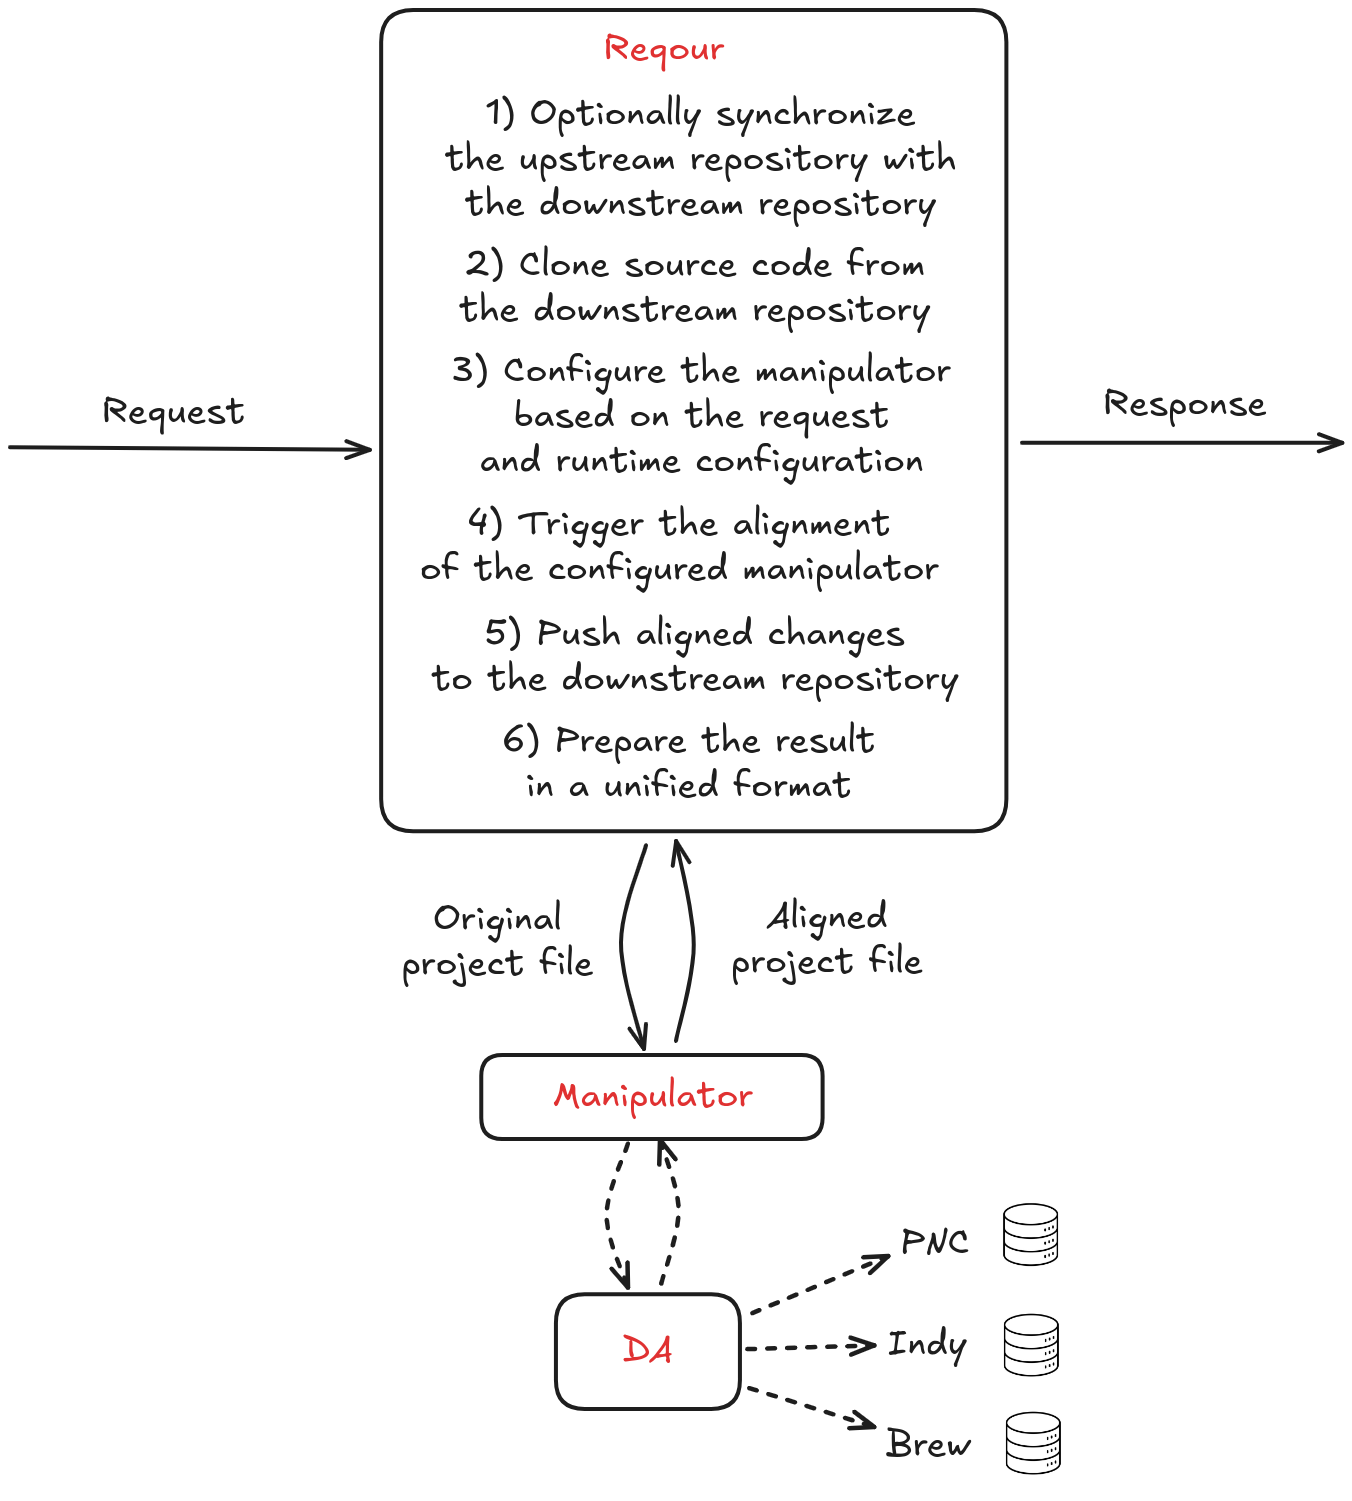
\includegraphics[width=\textwidth]{images/alignment-process.png}
  \end{center}
  \caption{High-level overview of alignment process}
  \label{fig:alignment-process}
\end{figure}

\textbf{Note:} By \textbf{alignment operation}, we mean both \textbf{version increment} together with \textbf{dependency alignment}. The difference between the two is that during a version increment, \textbf{next non-existing version} in the sequence is chosen, whilst during the latter, \textbf{the most feasible version from existing versions} is chosen.

\textbf{Example:} Suppose that we request DA and all available versions of the artifact \textit{org.foo:bar} are as shown in Figure \ref{fig:version-increment-vs-dependency-alignment}. Version increment for a temporary build will be \textbf{temporary-redhat-00003}. Dependency alignment for a persistent build will be \textbf{redhat-00003}\footnote{Supposing that simply the built artifact from the last persistent build is taken. In reality, PNC dependency alignment is a little more involved but it is not important for our context.}.

\begin{figure}
  \begin{center}
    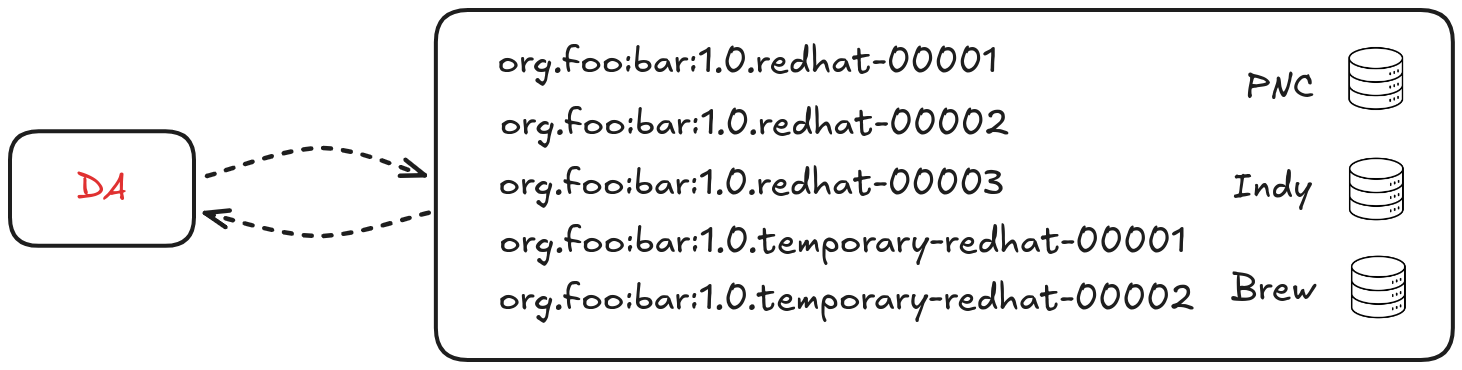
\includegraphics[width=\textwidth]{images/version-increment-vs-dependency-alignment.png}
  \end{center}
  \caption{DA and all available versions for the artifact \textit{org.foo:bar}}
  \label{fig:version-increment-vs-dependency-alignment}
\end{figure}

Finally, the table \ref{table:build-types-and-manipulators} lists build types and their corresponding manipulators used during alignment. Every manipulator but SMEG is distributed as a standalone JAR (SMEG being distributed as a Scala plugin). Maven and Gradle builds make up the vast majority of PNC builds. This results in PME and GME providing more functionalities. For instance, PME is the project maintained by \href{https://github.com/release-engineering}{Red Hat Productization}.

\begin{figure}
    \begin{center}
    \begin{tabular}{ |c|c| }
    \hline
    Build Type & Manipulator \\
    \hline
    Maven & \href{https://github.com/release-engineering/pom-manipulation-ext}{PME} \\ 
    Gradle & \href{https://github.com/project-ncl/gradle-manipulator}{GME} \\ 
    NPM & \href{https://github.com/project-ncl/project-manipulator}{Project Manipulator} \\ 
    SBT & \href{https://github.com/project-ncl/smeg}{SMEG} \\
    \hline
    \end{tabular}
    \end{center}
    \caption{Build types and corresponding manipulators}
    \label{table:build-types-and-manipulators}
\end{figure}

\end{document}
